\section{Grafici ed immagini}
\begin{figure}[h]
	\centering
	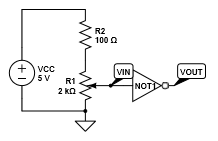
\includegraphics[scale=1]{circuito1.png}
	\caption{Circuito NOT}
	\label{f:circuito1}
\end{figure}
\begin{figure}[h]
	\centering
	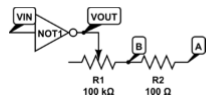
\includegraphics[scale=1]{circuito2.png}
	\caption{Circuito utilizzato per la misura delle correnti in uscita.}
           \label{f:circuito2}
\end{figure}

\begin{figure}[h]
	\centering
	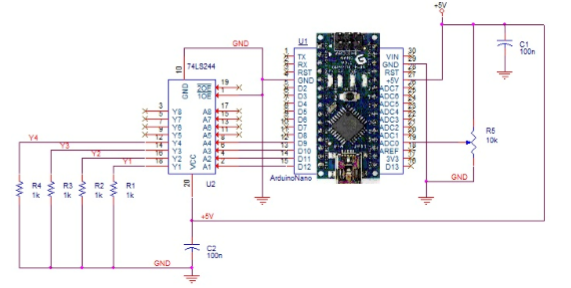
\includegraphics[scale=1]{arduino.png}
	\caption{Schema circuitale dell'impulsatore con microcontrollore Arduino}
           \label{f:Circuito}
\end{figure}

\begin{figure}[h]
	\centering
	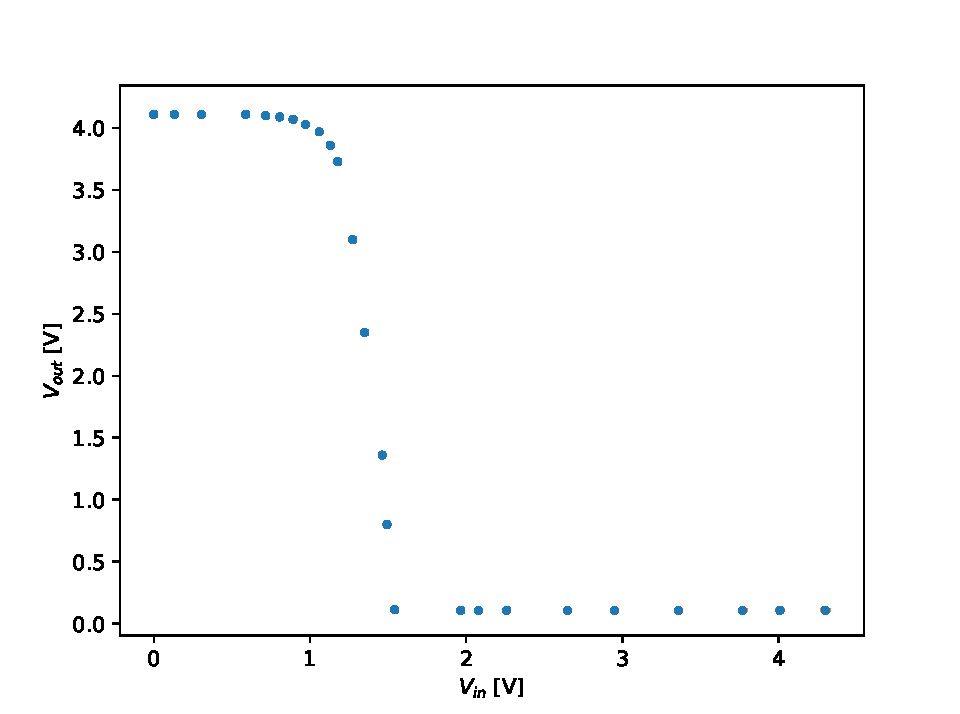
\includegraphics[scale=1]{out_in.pdf}
	\caption{Tensione in uscita in funzione della tensione in ingresso per la porta NOT}
           \label{f:out_in}
\end{figure}
\begin{figure}[h]
	\centering
	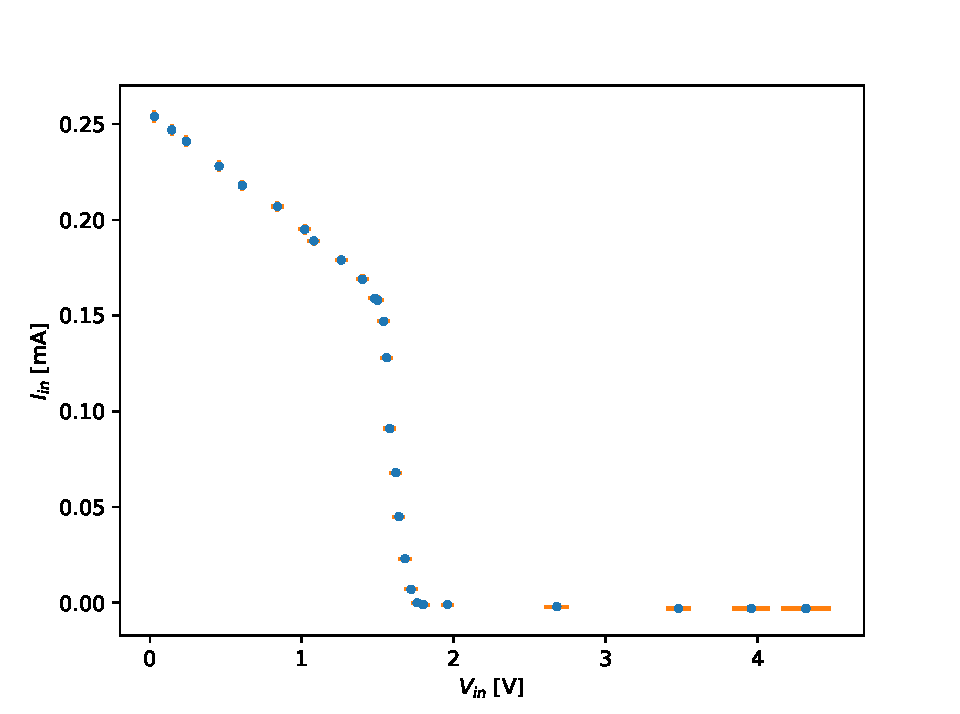
\includegraphics[scale=1]{Iout_in.pdf}
	\caption{Corrente in uscita in funzione della tensione in ingresso per la porta NOT}
           \label{f:Iout_in}
\end{figure}